\documentclass[../../../../main.tex]{subfiles}
\begin{document}

$AD$ と $BC$ が平行な台形 $ABCD$ を考える．

\begin{figure}[htbp]
  \centering
  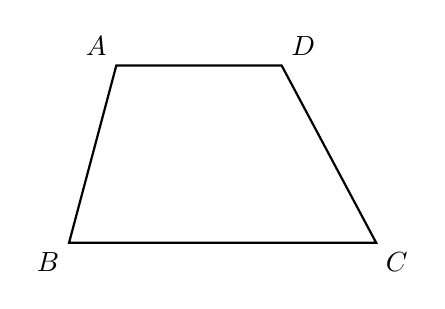
\begin{tikzpicture}[scale=1.5]
    \coordinate (A) at (0.4, 1.5);
    \coordinate (D) at (1.8, 1.5);
    \coordinate (B) at (0, 0);
    \coordinate (C) at (2.6, 0);

    \draw[thick] (A) -- (D) -- (C) -- (B) -- cycle;

    \node[above left] at (A) {$A$};
    \node[above right] at (D) {$D$};
    \node[below left] at (B) {$B$};
    \node[below right] at (C) {$C$};
  \end{tikzpicture}
\end{figure}

\begin{enumerate}
  \item 辺 $AB$ 上の点 $P$ と辺 $CD$ 上の点 $Q$ が線分 $PQ$ によって台形 $ABCD$ の面積を二等分するとき，$PQ$ の長さを求めよ．
\end{enumerate}

\end{document}
